\chapter{Event-based Reconfiguration Control Strategy for Time-varying Robot Formation in Confined Spaces}\label{paper2}

\noindent{\normalsize Published in:\\
\textit{Preprint}, 2024\\
% DOI:
}
\vspace{1cm}

\noindent\textit{\textbf{Abstract}}
Formation control plays a key role in coordinating multi-robot systems, especially in confined space environments where the risk of collisions is increased due to limited space. In this paper, we propose an event-based reconfiguration control (ERC) based on an artificial potential field that enhances the safety of time-varying robot formation (TVF) in a confined space. The proposed strategy includes two primary modes, \textit{``Formation''} and \textit{``Taigating''}, and provides flexible reconfiguration between original configuration and the straight-line configuration based on environmental perception. The proposed approach ensures that multi-robot systems maintain their desired configuration and collision-free trajectory. When a confined space is found to be insufficient to maintain the original formation, the configuration is either scaled down or transformed into a straight-line topology to maintain collision-free motion. A number of simulations, comparisons, and evaluations based on several metrics have been conducted to confirm the validity and superiority of the proposed approach.

\noindent\textbf{\textit{Keywords:}}
multi-robot system, time-varying formation, reconfiguration control, obstacle avoidance, event-triggering, artificial potential fields
% \end{keywords}

\section{Introduction}

With advancements in networked multi-agent technology, multi-robot systems (MRSs) have rapidly developed towards autonomy, offering various applications from warehouse automation to search and rescue operations~\cite {6303906,1335496}. A core element of these systems is a formation controller that enables the robots to collaborate in a desired configuration~\cite{1545539,Oh2015}. In rigid formation control, achieving the desired configuration involves setting a specific target distance for each swarm agent. However, with the increasing complexity of formation tasks, the formation configuration needs to be adjustable to meet specific task requirements. Time-varying formation (TVF) control thus has become essential for swarm robots~\cite{Dong2015,Dong2016}.

\begin{figure}
\centering
\begin{subfigure}[b]{0.4\textwidth}
    
    \centering
    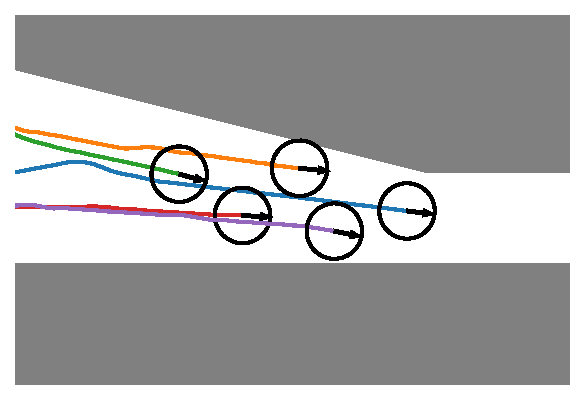
\includegraphics[width=\linewidth]{paper2/images/sample_bc.pdf}
    \caption{Pure formation control}
    \label{fig:1sample_bc}
\end{subfigure}
\begin{subfigure}[b]{0.4\textwidth}
    \centering
    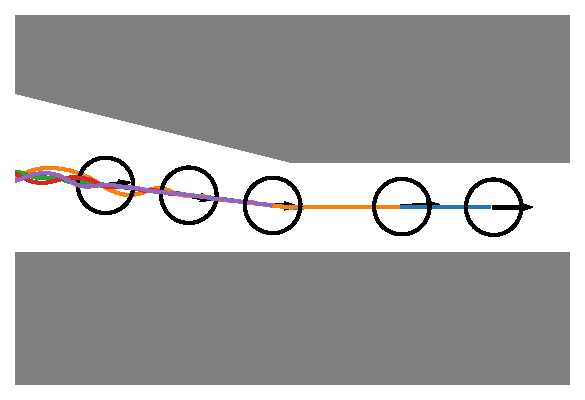
\includegraphics[width=\linewidth]{paper2/images/sample_edc.pdf}
    \caption{Proposed approach}
    \label{fig:1sample_edc}
\end{subfigure}
\caption{We develop an event-based reconfiguration control (ERC) method to guide a TVF through narrow spaces. \textit{Left:} Motion path of the TVF using purely behavior-based formation control~\cite{736776, Vsrhelyi2018}, which is collision with surrounding obstacles. \textit{Right:} Motion path of the TVF using our proposed approach, which safely navigates through the narrow spaces.}
\label{fig:1sample}
\end{figure}

Studies in~\cite{736776,Reynolds1987,Antonelli2009} show that biological swarm motion can be characterized by three primary behavioral rules: (i) \textit{cohesion}, which drives an agent toward to its neighbors; (ii) \textit{repulsion}, which pushes an agent away from its neighbors to prevent collisions; and (iii) \textit{alignment}, which aligns an agent to the dominant heading of its neighbors. For goal-oriented swarm motion, \textit{alignment} can be replaced by a \textit{migration} behavior so that each agent is directed in a desired orientation and moves at a preferred speed~\cite{6095129}. In complex environments, a fourth behavior called \textit{collision avoidance} can be added to guide the agent around obstacles~\cite{9565893, 9990164,1605401,10417519}. These behavioral rules are typically integrated into multi-robot systems through virtual forces within the artificial potential field (APF) to achieve coordinated movements~\cite{9981858,9561902,9990164}. Specifically, the APF has been used in~\cite{10417519,8716301,9565893} to navigate robot swarms through different environments, from open spaces to environments containing concave obstacles. In~\cite{9565893}, a fuzzy controller is added to allow the robot swarm to avoid complex obstacles while maintaining swarm connectivity. In~\cite{Vsrhelyi2018}, evolutionary optimization is combined with a behavioral model to enable stable and decentralized navigation for large-scale aerial robot swarms in confined spaces. However, using a fixed set of behaviors limits the flexibility of the swarm formation in response to abrupt changes in the environment, especially in spaces such as caves, corridors, and tunnels, and hence increases the risk of collisions~\cite{Saska2020,AlonsoMora2017}.

Apart from the behavior-based approach, studies in formation control can be further grouped into two primary categories: \textit{rigid formation}~\cite{Saska2020,Gmez2013,Roy2018,Ebel2017} and \textit{adaptive formation}~\cite{Fu2020,8843165,AlonsoMora2017,AlonsoMora2018}. In \textit{rigid formation}, the swarm can shrink or expand in size while preserving its overall shape. In~\cite{Saska2020}, a model predictive control is employed for rigid formation in which optimal control signals are generated for each robot in the swarm based on a shared map. In~\cite{Roy2018}, a region-based hierarchical control method is introduced for obstacle avoidance in confined spaces. The controller drives the robots to move cohesively within a virtual circular region that can contract to navigate around obstacles. A comprehensive control scheme is presented in~\cite{Ebel2017} for omnidirectional mobile robots to transport a plate through unknown environments collaboratively. The scheme uses graph-based path planning for obstacle avoidance and distributed model predictive control for optimal motion. Although rigid formations work well in open-space environments, they become ineffective in narrow spaces where the width of the space and the size of the formation directly affect navigation success. This challenge becomes critical when contracting the formation increases the risk of collision among the robots, as illustrated in Figure~\ref{fig:1sample_bc}.

In \textit{adaptive formation}, the swarm can transform into different configurations in adaptation to environmental conditions. In~\cite{Fu2020}, a reconfiguration strategy is combined with behavioral control for swarm navigation in dynamic environments. The strategy uses an auction-based market approach to generate solutions for formation movement. In~\cite{8843165}, particle swarm optimization is used to generate trajectories for a swarm of unmanned aerial vehicles (UAVs) that can reconfigure its formation for obstacle avoidance and task accomplishment. However, this approach is centralized and requires considerable computational resources to maintain an optimal configuration in real time. A robust adaptive formation control algorithm is introduced in~\cite{Mung2019} for a group of UAVs. The controller can steer the vehicles to form and maintain different formation patterns for flexible navigation. Generally, the adaptive formation methods are effective in guiding robots through complex environments as they enable flexible reconfiguration in response to environmental changes. However, there remains a need for a distributed, partial communication solution that ensures safe, efficient formation navigation while adapting effectively to environmental change.

In this work, we propose an event-based reconfiguration controller (ERC) for safe and effective navigation of a decentralized TVF in narrow environments, as given in Figure~\ref{fig:1sample}. The robots are equipped with local sensors and communication modules to collect information about the environment and other robots in the formation. The main contributions of this study are threefold:
\begin{enumerate}
    \item Define a set of individual behaviors that meet the reconfiguration control requirements, including goal-directed motion, formation maintenance, tailgating, and collision avoidance behaviors. Each behavior is designed for convenience in implementation via an artificial potential field.
        \item Propose an event-based reconfiguration controller with two modes, \textit{``formation''} and \textit{``tailgating''} capable of adapting the formation shape in response to environmental changes. The stability of the proposed approach has been demonstrated via the Lyapunov theorem.
    \item Extensive simulations and comparisons have been conducted to evaluate the robustness, scalability, and effectiveness of the proposed controller. Software-in-the-loop tests have also been conducted to verify its practical applicability. The source code of the proposed controller is publicly available for further research and practical implementation.
\end{enumerate}

The remaining sections of this paper are organized as follows. Section~\ref{sec2} presents the formation model and formulation. Section~\ref{sec3} introduces the proposed event-based reconfiguration control method. Simulation, comparison, and software-in-the-loop experimental results are shown in Section~\ref{sec4}. The paper ends with conclusions drawn in Section~\ref{sec5}.
\section{Preliminaries}\label{sec2}
\subsection{Model of robots}
Consider a swarm $\mathcal{N}$ that contains $n$ robots labelled $i\in\left\{1,...,n\right\}$. We model the swarm as a directed sensing graph $\mathcal{G}=\left(\mathcal{V},\mathcal{E}\right)$, where vertex set $\mathcal{V} = \left\{1,..., n\right\}$ represents the robots, and edge set $\mathcal{E}\subseteq\mathcal{V}\times \mathcal{V}$ contains the pairs of robots $\left(i, j\right)\in\mathcal{E}$ for which robot $i$ can sense robot $j$. We denote $\mathcal{N}_i=\left\{j\in\mathcal{V}|\left(i,j\right)\in\mathcal{E}\right\}\subset\mathcal{V}$ as the set of $n_i$ neighbours of a robot $i$ in $\mathcal{G}$.

\begin{figure}
    \centering
    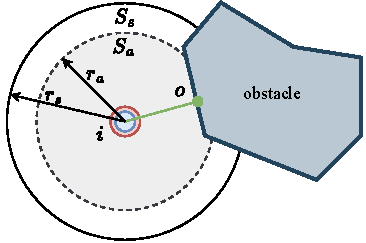
\includegraphics[width=0.45\textwidth]{paper2/images/model.pdf}
    \caption{Illustration of a robot with a local range sensor. Each robot is equipped with a local sensor with sensing area $S_s$ (solid while circle) being a circular disk within radius $r_s$. Additionally, alert area $S_a$ (dashed gray circle) is a circular disk within radius $r_a$, with $r_a\leq r_s$, which is the zone that robot will active the repulsive force to avoid collision. The set~$\mathcal{M}_i=\{o\}$ (green) is the nearest point from robot $i$ to obstacle.}
    \label{fig:1model}
\end{figure}

\begin{figure*}
    \centering
    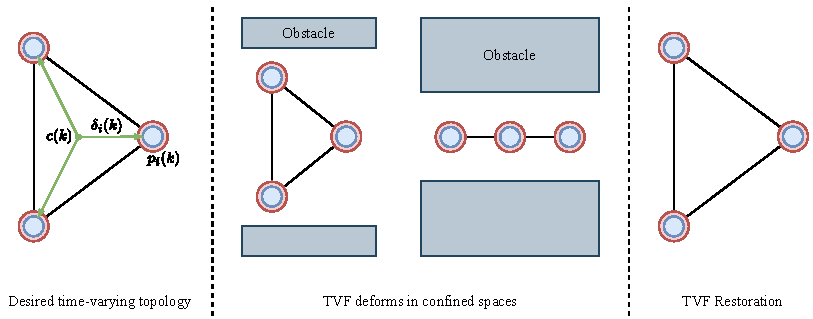
\includegraphics[width=0.9\textwidth]{paper2/images/problem.pdf}
    \caption{Schematic diagram of time-varying formation in the confined space}
    \label{fig:1problem}
\end{figure*}
In this study, the robots' dynamics are expressed in discrete time. The position, velocity, and control input of robot $i$ at time $t(k) = k\tau$ are denoted as $p_i(k), v_i(k), u_i(k) \in \mathbb{R}^3$, respectively, where $\tau$ represents the time step. The robots in the swarm are identical, each with a body radius $r$. Each robot $i$ is equipped with an inertial measurement unit (IMU) to determine its position and orientation in a desired direction, a range sensor, and a wireless ad-hoc network module for peer-to-peer communication with other robots. In this study, the communication delay between any two robots is assumed to be negligible~\cite{AlonsoMora2018,9527169}. Additionally, each robot is equipped with a circular sensor~\cite{8716301} that offers a $360^\circ$ field of view of the environment and can observed a maximum area $S_s$ within a radius $r_s$, as depicted in Fig.~\ref{fig:1model}. The set $\mathcal{M}_i(k) = \left\{o\right\}$ represents the observed obstacle points $o$ which is the nearest point on the obstacle's boundary at time $t(k)$. Additionally, a circular with the radius $r_a$ is denoted as an alert area that actives repulsive forces when robot $i$ sensing obstacles or its neighbors.

According to~\cite{Dong2015}, assuming that every robot in the swarm obeys a discrete linear system, given by
\begin{equation}
    x_i(k+1)=A_ix_i(k) + B_iu_i(k)
    \label{eqn:1model}
\end{equation}
where $A_i$ and $B_i$ are constant matrices. We consider the system to represent a robot with an underlying acceleration controller. The input $u_i$ is an acceleration command, and the state $x_i=\left[p_i,v_i\right]^T\in\mathbb{R}^6$ is a vector containing the position and velocity. The velocities and accelerations of the robots are bounded by constant vectors, i.e. $\left\Vert v_i(k)\right\Vert\leq v_\text{max}$ and $\left\Vert u_i(k)\right\Vert\leq u_\text{max}$.

\subsection{Problem formulation}

This paper addresses the safe formation control of time-varying formation (TVF) in confined space. The primary challenges addressed are:
\begin{enumerate}
    \item Ensuring collision-free navigation for the TVF, even when in the limited space environment.
        \item Incorporating an event-triggering mechanism into the TVF control, allowing the formation to deform to another safe configuration.
\end{enumerate}

Fig.~\ref{fig:1problem} provides the general schematic diagram of the research problem tackled in this study. Initially, the desired configuration assigned to the TVF is denoted $\delta_0$. At time $k$, the TVF can maintain the initial topology, i.e. $\delta(k)=\delta_0$. However, the confined space does not allow the formation maintaining topology $\delta_0$ due to the potential collision. As a result, a new topology is triggered to be applied depending on the surrounding space. Once the confined space is not detected by the robot, the initial topology $\delta_0$ of the formation is restored. With the proposed control approach, the formation configuration can be effectively managed. During the movement of the TVF, collaborative and collision avoidance controls are driven by the APF term in the proposed control strategy.

\begin{definition}\label{def_tvf}
(Time-Varying Formation~\cite{Dong2015,Dong2016} - TVF).  Let $\delta(k)=\left[\delta_1(k),...,\delta_n(k)\right]^T$ be a bounded time-varying vector that describes the desired formation configuration. The formation is said to achieve a TVF $\delta(k)$ if all robot $i$ in the formation satisfy:
\begin{equation}
    \lim_{k\to\infty}\sum_{i=1}^n\left\Vert p_i(k)-\delta_i(k)-c(k)\right\Vert=0,\quad\forall i\in\left\{1,...,n\right\}
\end{equation}
where $c(k)$ is called a formation center in the time $k$.
\end{definition}

\begin{definition}\label{def_pro}
(Safe Formation Control). Given the TVF as defined in Definition~\ref{def_tvf}, the safe formation control of TVF is said to be realized for any robot $i$ in the formation if the following conditions are simultaneously satisfied:
\begin{enumerate}
    \item Formation configuration
\begin{equation}
    \lim_{k\to\infty}\sum_{i=0}^n{\left\Vert\left(p_i(k)-\delta_i\right) - \left(p_j(k)-\delta_{j}\right)\right\Vert}=0
    \label{eqn:1form}
\end{equation}
for all $i,j\in\left\{1,...,n\right\}$, $i\neq j$.
%     \item Task completion
% \begin{equation}
%     \lim_{k\to T}\left\Vert\dfrac{1}{n}\sum_{i=1}^np_i-p_g\right\Vert=0
%     \label{eqn:1goal}
% \end{equation}
% where $T$ is a finite time, $p_g$ is the target position.
    \item Safe distance between robots
\begin{equation}
    \left\Vert p_i(k)-p_j(k)\right\Vert > 2r
    \label{eqn:1col}
\end{equation}
for all $i\in\left\{1,...,n\right\}$.
    \item Safe distance from obstacles
\begin{equation}
    \left\Vert p_i(k)-m\right\Vert > r
    \label{eqn:1obs}
\end{equation}
for all $i\in\left\{1,...,n\right\}$, and for all $m\in\mathcal{M}_i(k)$. 
\end{enumerate}
\end{definition}

\begin{remark}
According to the discrete linear model presented in~\eqref{eqn:1model}, this study primarily focuses on the changes in the position and velocity status of the robot. Based on Definition~\ref{def_tvf}, when~\eqref{eqn:1form} is established, robots reach the desired position, achieving the desired configuration. 
% Simultaneously, the velocity tends to zero once the tasks are completed~\eqref{eqn:1goal}. 
The establishment of \eqref{eqn:1col}~--~\eqref{eqn:1obs} ensure that the robot will not collide with obstacles or other robots in the formation, respectively.
\end{remark}

\subsection{Formation configurations}\label{sec:config}
Formation configurations are emerging while robots are cooperating and interacting with the confined space environments. In this study, we categorize formation configurations into two primary configurations:
\begin{enumerate}
    \item \textit{Original configuration:} This formation configuration is maintained if any surrounding space is large enough to maintain the originally defined configuration or to transform it by contraction. The configuration can be a V-shape, a polygon, or others.
        \item \textit{Straight line configuration:} This formation configuration is performed when the robot does not have enough space to maintain the original configuration, forcing it convert to this form for safety assurance~\cite{Fu2020}. This configuration is constructed by having a robot follow and keep desired distance from its leader.
\end{enumerate}
\section{Event-based Reconfiguration Control}\label{sec3}

To address the TVF problem, several potential force-based behaviors for each robot $i$ are used to synthetic to the proposed controller, which contains emergent strategies to navigate TVF to deal with the narrow space environment while ensuring the shape and the safety of TVF, named \textit{``formation''}, and \textit{``tailgating''}. In \textit{``formation''} mode, the TVF maintains the original configuration, while in \textit{``tailgating''} mode, the TVF transforms to the straight line configuration, as presented in Section~\ref{sec:config}. The detail of the proposed strategies is described in Figure~\ref{fig:1control_diagram}.

\begin{figure*}
    \centering
    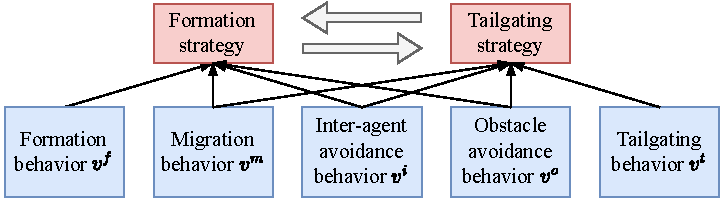
\includegraphics[width=0.85\textwidth]{paper2/images/control_diagram.pdf}
    \caption{Overview of the proposed event-based reconfiguration control. The proposed strategy is constructed by two primary emergent strategy, including \textit{``formation''} and \textit{``tailgating''}, which are highlighted by red boxes. There are five individual behaviors that contribute to the emergent strategy, which illustrated via blue boxes.}
    \label{fig:1control_diagram}
\end{figure*}

Our approach incorporates an event-triggering mechanism into the TVF that allows the swarm to adapt its formation shape in response to environmental conditions for safe navigation, as illustrated in Figure~\ref{fig:1problem}. Initially, the desired configuration assigned to the TVF is denoted $\mathbf{\delta}_0$. At time $k$, the TVF can maintain the initial topology, i.e. $\mathbf{\delta}(k)=\mathbf{\delta}_0$. However, the confined space does not allow the formation maintaining topology $\mathbf{\delta}_0$ due to the potential collision. As a result, a new topology is triggered to be applied depending on the surrounding space. Once the confined space is not detected by the robot, the initial topology $\mathbf{\delta}_0$ of the formation is restored. With the proposed control approach, the formation configuration can be effectively managed. During the movement of the TVF, collaborative and collision avoidance controls are driven by the APF term in the proposed control strategy.

\subsection{Individual behaviors}
According to~\cite{Vsrhelyi2018}, the potential field model is used to design individual behaviors a state-of-the-art model that allows robot swarm navigation in confined environments. From the original model, we design the rule of attraction for formation maintenance, tailgating and goal orientation; the rule of repulsion to prevent inter-robot collisions, and obstacle avoidance to avoid collisions with 
obstacles. 

Firstly, to ensure goal-directed motion in environments, a target reaching behavior is provided by a preferred velocity vector. We denote $v_\text{ref}$ is the preferred speed and $\mathbf{u}_\text{ref}$ is the preferred direction~\cite{6095129}. Then, the migration term, equal for every agent, corresponds to:
\begin{equation}
    \mathbf{v}_i^m=v_\text{ref}\mathbf{u}_\text{ref}
\end{equation}

Secondly, the formation behavior is designed as an attractive force that drive robots to move toward their desired positions. Denote $\kappa\in\mathbb{R}$ be the scale ratio, which can be determined in Section~\ref{sec:erc}. Thus, a relative position-based controller of the form to maintain the desired shape, and enhance the abilities of TVF with scalable capabilities, which is given as follow:
\begin{equation}
    \mathbf{v}^f_i=k_f\sum_{j=1}^n{\left(\mathbf{p}_j-\mathbf{p}_i-\kappa\left(\mathbf{\delta}_j-\mathbf{\delta}_i\right)\right)}
    \label{eqn:1uf}
\end{equation}
where $k_f>0$ is the formation control gain.

Next, the tailgating behavior is designed based on the relative position between each robot with other robot in the TVF, and used to navigate TVF pass through the narrow environment. Let robot $i$ follows robot ${l_i}$ within desired distance $d_\text{ref}$, with $d_\text{ref}>2r$,  an attractive force field for robot $i$ can be expressed as follows:
\begin{equation}
    \mathbf{v}_i^t=\begin{cases}
k_t\left(\mathbf{p}_{l_i}-\mathbf{p}_i-d_\text{ref}\dfrac{\mathbf{v}_{l_i}}{\left\Vert \mathbf{v}_{l_i}\right\Vert}\right)+\mathbf{v}_{l_i} & \text{if } l_i\neq-1\\
0 & \text{otherwise}
\end{cases}
    \label{eqn:1ut}
\end{equation}
where $k_t$ is the tailgating control gain. To determine the leader robot, the inner product $\tilde{\mathbf{p}}_{ij}$ of the difference between robot $j$ in the neighbor set $\mathcal{N}_i$ with robot $i$, $\mathbf{p}_j-\mathbf{p}_i$, and the desired direction, $\mathbf{u}_\text{ref}$, is given as follows:
\begin{equation}
    \tilde{\mathbf{p}}_{ij} = \left\langle (\mathbf{p}_j-\mathbf{p}_i),\mathbf{u}_\text{ref}\right\rangle
    \label{eqn:1tildep}
\end{equation}

As a result, the value of $\tilde{\mathbf{p}}_{ij}$ is positive, proving that robot $j$ is in front of robot $i$ according to $\mathbf{u}_\text{ref}$, and vice versa. For all robots $j$ in swarm, we obtain $\mathcal{P}_i=\left\{\tilde{\mathbf{p}}_{ij}\right\}$. The leader robot ${l_i}$ of robot $i$ is chosen as the closest robot in front of it, i.e.
\begin{equation}
     l_i=\begin{cases}
    \arg\min_{j}\left\{\tilde{\mathbf{p}}_{ij}\in\mathcal{P}_i\vert\tilde{\mathbf{p}}_{ij}\geq0\right\} & \exists~\tilde{\mathbf{p}}_{ij}\geq0\\ 
    -1 & \text{otherwise}
     \end{cases}
    \label{eqn:1li}
\end{equation}

Finally, inter-agent avoidance and obstacle avoidance behaviors are also designed to prevent collision. Denote $\mathcal{M}_i$ be the set of finite points on the obstacle's boundary, which are the closest to robot $i$, as illustrated in Figure~\ref{fig:1model}. Those repulsive forces are given as follows:
\begin{equation}
    \mathbf{v}_i^i=k_{i}\sum_{j=1,j\neq i}^n{\mathbf{v}_{ij}^i}
\end{equation}
\begin{equation}
    \mathbf{v}_i^o=k_o\sum_{\mathbf{o}\in\mathcal{M}}\mathbf{v}_{io}^o
\end{equation}
where $k_i,k_o>0$ is the inter-agent collision and obstacle avoidance gains, respectively. Denote $\mathbf{p}_{ij}=\mathbf{p}_i-\mathbf{p}_j$, and $\hat{\mathbf{p}}_{ij}=\dfrac{\mathbf{p}_{ij}}{\left\Vert \mathbf{p}_{ij}\right\Vert}$ be the relation position and the normalized vector between robot $i$ and robot $j$, respectively. Similarly, $\mathbf{p}_{io}$, and $\hat{\mathbf{p}}_{io}$ are the relative position and the normalized vector between robot $i$ and obstacle $\mathbf{o}$, respectively, with $\mathbf{o}\in\mathcal{M}_i$. Thus, the associated inter-agent avoidance $\mathbf{v}_{ij}^i$ and obstacle avoidance $\mathbf{v}_{io}^o$ are given as follows:
\begin{equation}
    \mathbf{v}_{ij}^{i}=\begin{cases}
    \dfrac{r_a-\left\Vert \mathbf{p}_{ij}\right\Vert}{r_a -2r}\hat{\mathbf{p}}_{ij} & \text{if }\left\Vert \mathbf{p}_{ij}\right\Vert<r_{a} \\
    0 & \text{otherwise}
    \end{cases}
    \label{eqn:1ui}
\end{equation}
\begin{equation}
    \mathbf{v}_{io}^{o}=\begin{cases}
    \dfrac{r_a-\left\Vert \mathbf{p}_{io}\right\Vert}{r_a -r}\hat{\mathbf{p}}_{io} & \text{if }\left\Vert \mathbf{p}_{io}\right\Vert<r_{a} \\
    0 & \text{otherwise}
    \end{cases}
    \label{eqn:1uo}
\end{equation}

\subsection{Event-based Reconfiguration Control strategy}\label{sec:erc}

As mentioned in Figure~\ref{fig:1control_diagram}, the proposed event-based reconfiguration control includes two emergent strategies to navigate TVF safely through narrow space environment while maintaining the shape and ensuring the safety of swarm. At each time step, each robot determine the mode itself based on the sensing data collected from local sensor. The overall strategy can be summarised as follows:
\begin{equation}
    \tilde{\mathbf{v}}_i=\begin{cases}
        \mathbf{v}_i^f+\mathbf{v}_i^m+\mathbf{v}_i^c+\mathbf{v}_i^o & \text{if mode = \textit{``formation''}}\\
        \mathbf{v}_i^t+\mathbf{v}_i^m+\mathbf{v}_i^c+\mathbf{v}_i^o & \text{if mode = \textit{``tailgating''}}
    \end{cases}
    \label{eqn:1v}
\end{equation}

To search the large parameter space $\Xi=\left\{k_f,k_t,k_i,k_o\right\}$ of the controller, evolutionary optimization can be used for highest-order flight and lowest number of collisions. The evaluation of the swarm behavior is based on a single fitness function that sums three independent values, including order, agent-safety, and obs-safety, smaller or equal to 1 (ideal case). The fitness is determined in simulations where the swarm is initialized with random positions in an environment where obstacles are  randomly placed. The description  to seek parameter values are similar and detailed in the~\cite{Vsrhelyi2018}.

To select the suitable mode at each time step, an event-based mode switching is designed to deal with the requirement to navigate a TVF through a narrow space environment. According to the individual behaviors and emergent strategies mentioned above, the mode of each robot can be changed based on its sense with environment around.

\begin{figure}
    \centering
    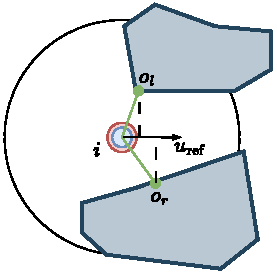
\includegraphics[width=0.35\textwidth]{paper2/images/we.pdf}
    \caption{Environment's width estimation}
    \label{fig:1we}
\end{figure}

Each obstacle point in the set $\mathcal{M}_{i}$ is clustered into two clusters on the left and right sides of the robot in $\mathbf{u}_\text{ref}$ direction. Denote $\mathbf{o}_l$ and $\mathbf{o}_r$ are the nearest obstacle points on the left and right sides, respectively, whose distance to the robot $i$ is minimum. If $\mathbf{o}_l$ and $\mathbf{o}_r$ exist, the width of the environment can be estimated by the magnitude of the cross product of the vector $(\mathbf{o}_r-\mathbf{o}_l)$ and the desired direction $\mathbf{u}_\text{ref}$ as follows:
\begin{equation}
    w_e= \left\Vert\left(\mathbf{o}_r-\mathbf{o}_l\right)\times \mathbf{u}_\text{ref}\right\Vert
    \label{eqn:1we}
\end{equation}

The estimation of the environment's width can be depicted in Figure~\ref{fig:1we}. Besides, the formation's width $w_f$ can be easily determined through the predefined formation topology. Given the widths of the environment and formation, the scaling factor $\kappa$, which contributes to \eqref{eqn:1uf}, can be computed as follows:
\begin{equation}
    \kappa = 
    \begin{cases} 
        \dfrac{w_e - 2r}{w_f} & \text{if } w_e \geq \lambda r \\
        0 & \text{otherwise}
    \end{cases}
    \label{eqn:1kappa}
\end{equation}

As a result, each robot $i$ can choose its mode and compute scaling factor $\kappa$. Denote $\lambda>2$ be the threshold to transform between two mode. As presented in Algorithm~\ref{alg:1our}, the desired velocity $\tilde{v}_i$ corresponding to its mode can be obtained.
\begin{algorithm}[h!]
\caption{Pseudocode of the ERC strategy}
\label{alg:1our}
Get a set of observed obstacle points $\mathcal{M}_i$\;
\If{$\mathcal{M}_i$ is empty}{
    mode $\leftarrow$ \textit{``formation''}\;
    $\kappa \leftarrow 1.0$\;
}
\Else{
    Determine the obstacle points $\mathbf{o}_l$, $\mathbf{o}_r$\;
    \If{$\nexists \mathbf{o}_l$ or $\nexists \mathbf{o}_r$}{
        mode $\leftarrow$ \textit{``formation''}\;
        $\kappa \leftarrow 1.0$\;
    }
    \Else{
        Get the space's width $w_e$\tcc*[r]{Eq. \ref{eqn:we}}
        \If{$w_e\leq\lambda r$}{
            mode $\leftarrow$ \textit{``tailgating''}\;
        }
        \Else{
            mode $\leftarrow$ \textit{``formation''}\;
            Estimate the desired formation width $w_f$\;
            \If{$w_e-2r\leq w_f$}{
                Compute the scaling factor $\kappa$\tcc*[r]{Eq. \ref{eqn:1kappa}}
            }
            \Else{
                $\kappa\leftarrow1.0$\;
            }
        }
    }
}
Compute desired velocity $\tilde{\mathbf{v}}_i$\tcc*[r]{Eq. \ref{eqn:1v}}
\Return $\tilde{\mathbf{v}}_i$\;
\end{algorithm}

After summing the contributions, we apply a cutoff on the acceleration at $u_\text{max}$ according to
\begin{equation}
    \mathbf{u}_i=\dfrac{\tilde{\mathbf{u}}_i}{\left\Vert\tilde{\mathbf{u}}_i\right\Vert}\min(\left\Vert\tilde{\mathbf{u}}_i\right\Vert, u_\text{max})
\end{equation}
where $\tilde{\mathbf{u}}_i(k+1) =(\tilde{\mathbf{v}}_i(k+1)-\tilde{\mathbf{v}}_i(k)) /\tau$. Then, we apply a cutoff on the speed at $v_\text{max}$, and get the velocity command $v_i$ as follows:
\begin{equation}
    \mathbf{v}_i=\dfrac{\tilde{\mathbf{v}}_i}{\left\Vert\tilde{\mathbf{v}}_i\right\Vert}\min(\left\Vert\tilde{\mathbf{v}}_i\right\Vert, v_\text{max})
\end{equation}

\subsection{Stability analysis}
\begin{theorem}\label{the:stability}
Given the TVF as described in~\eqref{eqn:1model}, under the control law given in \eqref{eqn:1v}, the TVF asymptotically converges to the desired configuration.
\end{theorem}
\begin{proof}
To prove Theorem~\ref{the:stability}, we consider the negligible effect of collision avoidance behaviors and also neglect the constant impact of migration behavior, for any time $t(k)$, thus we conduct a stability analysis of the TVF in main contributions, i.e. formation and tailgating behaviors, which located in two separate modes, \textit{``formation''} and \textit{``tailgating''}, as mentioned in Section~\ref{sec:config}, which together ultimately lead to our conclusion.

\textbf{Mode \textit{``formation''}:} Denote $L$ be the Laplacian matrix of the interaction topology graph of the swarm. Due to the fully connected, the entries of $\mathbf{L}=\left[l_{ij}\right]$ are given as follows:
\begin{equation}
    l_{ij}=\begin{cases}
    -1 & \text{if }i\neq j \\
    n-1 & \text{if }i=j
    \end{cases}
\end{equation}

The control law \eqref{eqn:1uf} can be shown as follows:
\begin{equation}
    k_f\sum_{j=1}^n{\left(\mathbf{p}_j-\mathbf{p}_i-\kappa \delta_{ji}\right)}=k_f\sum_{j=1}^n{\left(\mathbf{p}_j-\mathbf{p}_i\right)}+\mathbf{b}_i
\end{equation}
where the bias $\mathbf{b}_i=-k_f\sum_{j=1}^n\kappa \delta_{ji}$.  In order to use the properties of the Laplacian matrix, the dynamics of the swarm system with the control law can be expressed as follows:
\begin{equation}
    \dot{\mathbf{P}}=-k_f\mathbf{L}\mathbf{P}+\mathbf{B}
\end{equation}
where $\mathbf{P}=\left[\mathbf{p}_1,...,\mathbf{p}_n\right]^T$, $\mathbf{B}=\left[\mathbf{b}_1,...,\mathbf{b}_n\right]^T$ and $\mathbf{L}$ is the Laplacian matrix of the interaction topology graph of the formation. For these values of its elements the Laplacian matrix has only one zero eigenvalue and the rest of its eigenvalues are positive and the same. Note also that the vector $\mathbf{B}$ is an eigenvector of $\mathbf{L}$ with the corresponding eigenvalue $n$ and:
\begin{equation}
    \mathbf{L}\mathbf{B}=n\mathbf{B}
\end{equation}

Defined the Lyapunov-like function for the TVF system as follows:
\begin{equation}
    V_f=\dfrac{1}{2}\left(\mathbf{P}-\dfrac{1}{k_fn}\mathbf{B}\right)^T\left(\mathbf{P}-\dfrac{1}{k_fn}\mathbf{B}\right)
\end{equation}

Talking the first derivative of $V_f$ gives
\begin{equation}
\begin{aligned}
    \dot{V}_f&=\left(\mathbf{P}-\dfrac{1}{k_fn}\mathbf{B}\right)^T\left(-k_f\mathbf{L}\mathbf{P}+\mathbf{B}\right)\\
    &=-k_f\left(\mathbf{P}-\dfrac{1}{k_fn}\mathbf{B}\right)^T\mathbf{L}\left(\mathbf{P}-\dfrac{1}{k_fn}\mathbf{B}\right)\leq0
\end{aligned}
\end{equation}

According to the LaSalle’s invariance
principle, it can be stated that as $k\to\infty$ the state $\mathbf{P}$ will converge to the largest invariant subset $\Omega=\left\{\mathbf{P}|\dot{V}_f=0\right\}$. In other words, the formation will close to the desired shape.

\textbf{Mode \textit{``tailgating''}:} In case robot $i$ do not have it leader, we do not analysis the stability, because this robot do not contribute to the configuration maintenance of the TVF. Otherwise, in case robot $i$ has its leader $l_i$, we define a candidate Lyapunov function as follows:
\begin{equation}
    V_{t}=\dfrac{1}{2}\left(\mathbf{p}_{l_i}-\mathbf{p}_{i}-d_\text{ref}\dfrac{\mathbf{v}_{l_i}}{\left\Vert \mathbf{v}_{l_i}\right\Vert}\right)^{T}\left(\mathbf{p}_{l_i}-\mathbf{p}_{i}-d_\text{ref}\dfrac{\mathbf{v}_{l_i}}{\left\Vert \mathbf{v}_{l_i}\right\Vert}\right)
\end{equation}

Taking the first derivative of $V_t$, gives:
\begin{equation}
    \dot{V}_{t}=\left(\mathbf{p}_{l_i}-\mathbf{p}_{i}-d_\text{ref}\dfrac{\mathbf{v}_{l_i}}{\left\Vert \mathbf{v}_{l_i}\right\Vert}\right)^{T}\left(\mathbf{v}_{l_i}-\mathbf{v}_{i}\right)
\end{equation}

By using the control law $\mathbf{v}^t_i$ in \eqref{eqn:1ut}, $\dot{V}_t$ becomes:
\begin{equation}
    \dot{V}_{t}=-k_{t}\left(\mathbf{p}_{l_i}-\mathbf{p}_{i}-d_\text{ref}\dfrac{\mathbf{v}_{l_i}}{\left\Vert \mathbf{v}_{l_i}\right\Vert}\right)^{T}\left(\mathbf{p}_{l_i}-\mathbf{p}_{i}-d_\text{ref}\dfrac{\mathbf{v}_{l_i}}{\left\Vert \mathbf{v}_{l_i}\right\Vert}\right)\leq0
\end{equation}

Therefore, the Lyapunov stability is satisfied. That leads to robot $i$ converges to its leader $l_i$ and keep behind a distance $d_\text{ref}$ along its leader direction. As a result, the straight line configuration can be guaranteed.
\end{proof}

\begin{remark}
In the research of this chapter, decentralized control architecture is adopted for the TVF. Each robot in the formation can decide the mode itself based on information collected from the surrounding environment. The event-triggering condition designed in Algorithm~\ref{alg:1our} is also distributed and presented in the form of compact sets. Besides, the control law \eqref{eqn:1v} demonstrates stability based on Lyapunov theory. Under the action of the designed control law, the TVF will asymptotically achieve the desired configuration in both modes.
\end{remark}
\section{Results}\label{sec4}
\subsection{Simulation and Comparison}
\begin{figure*}[!h]
\begin{subfigure}[b]{\textwidth}
    
    \centering
    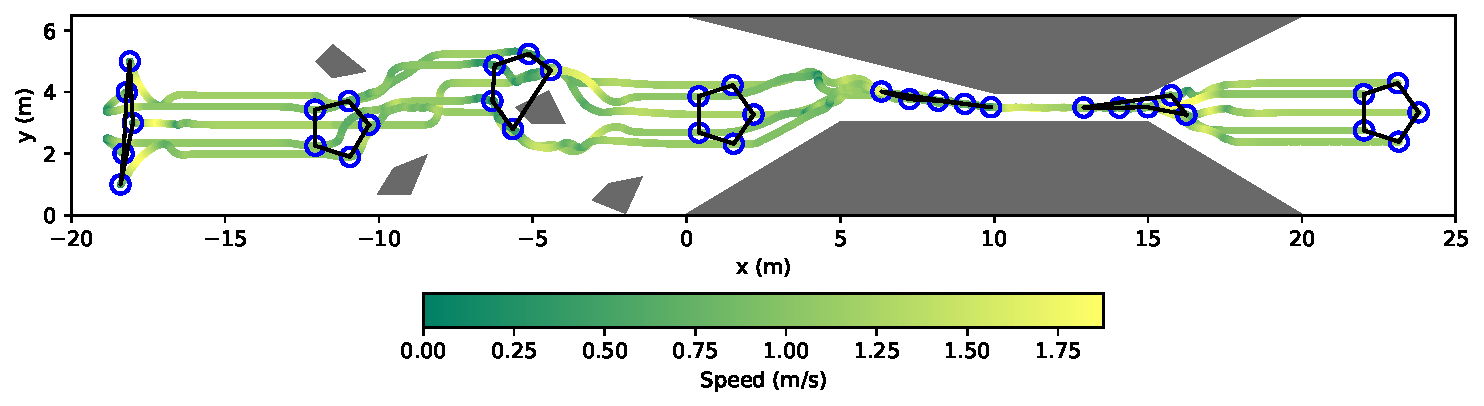
\includegraphics[width=0.9\textwidth]{paper2/images/path_edc_shape1.pdf}
    \caption{Pentagon configuration}
    \label{fig:1path_edc1}
\end{subfigure}
\begin{subfigure}[b]{\textwidth}
    \centering
    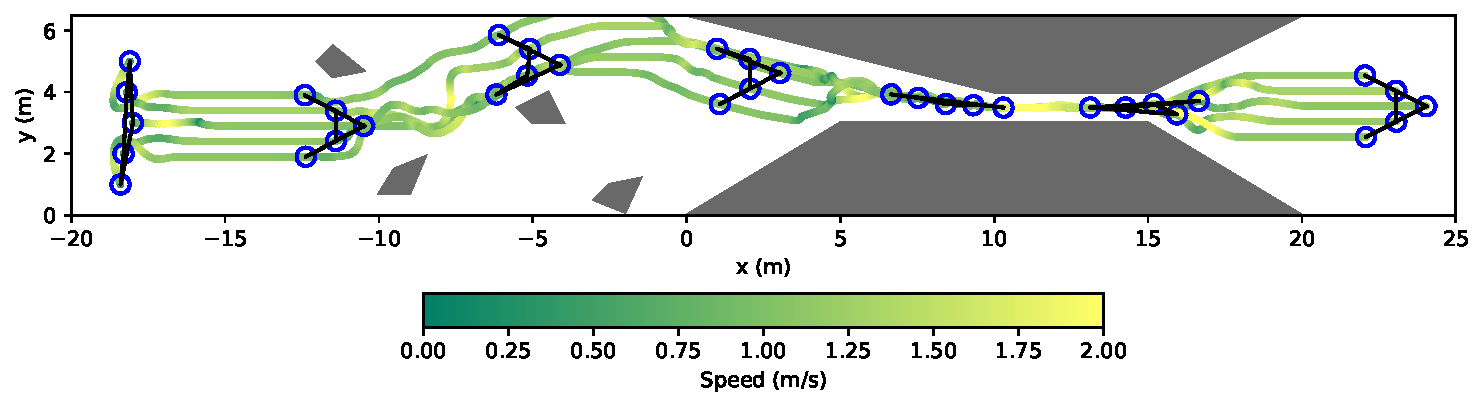
\includegraphics[width=0.9\textwidth]{paper2/images/path_edc_shape2.pdf}
    \caption{V-shape configuration}
    \label{fig:1path_edc2}
\end{subfigure}
\caption{Motion paths and velocity profiles of the proposed \textit{EFRC} strategy in multiple configurations.}
\label{fig:1path}
\end{figure*}

\begin{figure*}[!h]
\begin{subfigure}[b]{0.49\textwidth}
    
    \centering
    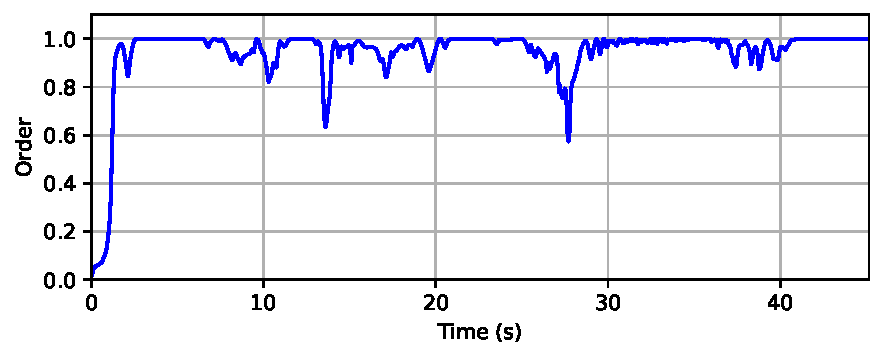
\includegraphics[width=\linewidth]{paper2/images/order_edc_shape1.pdf}
    \caption{Pentagon configuration}
    \label{fig:1order_edc1}
\end{subfigure}
\begin{subfigure}[b]{0.49\textwidth}
    \centering
    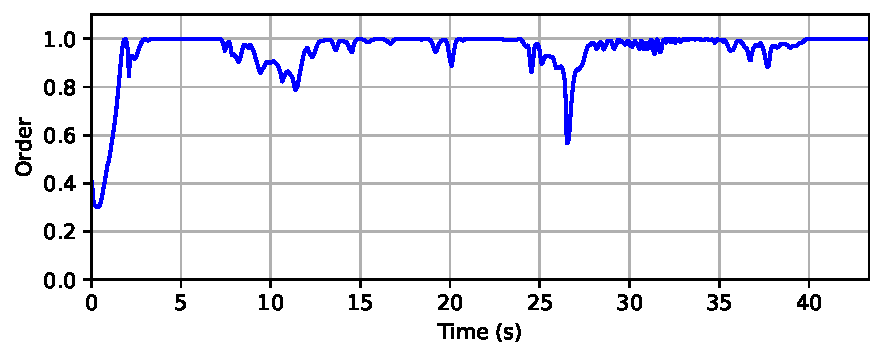
\includegraphics[width=\linewidth]{paper2/images/order_edc_shape2.pdf}
    \caption{V-shape configuration}
    \label{fig:1order_edc2}
\end{subfigure}
\caption{The \textit{order} values of the proposed \textit{EFRC} strategy}
\label{fig:1order}
\end{figure*}

\begin{figure*}[!h]
\begin{subfigure}[b]{0.49\textwidth}
    
    \centering
    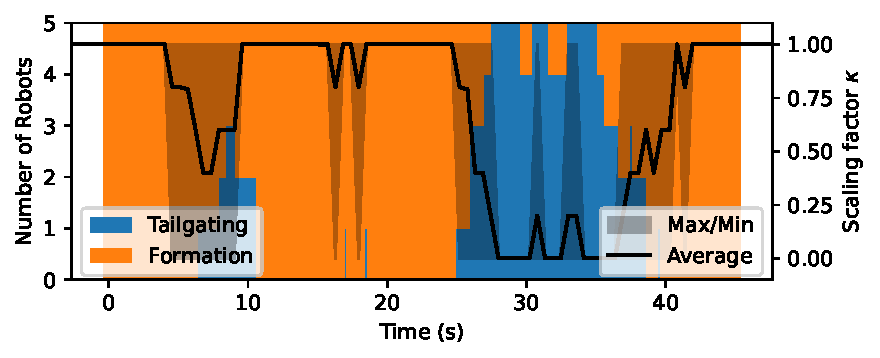
\includegraphics[width=\linewidth]{paper2/images/mode_edc_shape1.pdf}
    \caption{Pentagon configuration}
    \label{fig:1mode_edc1}
\end{subfigure}
\begin{subfigure}[b]{0.49\textwidth}
    \centering
    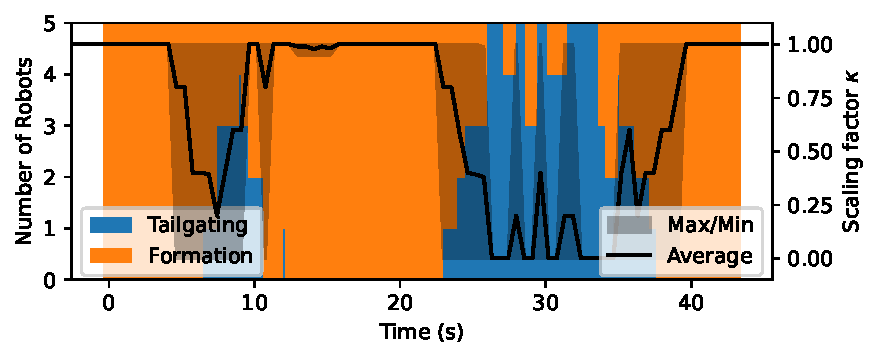
\includegraphics[width=\linewidth]{paper2/images/mode_edc_shape2.pdf}
    \caption{V-shape configuration}
    \label{fig:1mode_edc2}
\end{subfigure}
\caption{Correlation of number of robots and scaling factor of the proposed \textit{EFRC} strategy}
\label{fig:1mode}
\end{figure*}

% The simulations are run on AMD Ryzen 5 5500U with a base frequency of 2.1 GHz. 
The proposed strategy is tested in a complex environment, which consists of 2 areas of different obstacle types, one area is the forest-liked environment, whose obstacle densities is 0.05 obs/m$^2$ (for $-12$~m $<x<0$~m), another area is the width-varying cave-like environment with the most narrowed space is 1~m (for $0$~m $<x<20$~m). The TVF starts randomly from the left-hand side of the environment and has a mission to travel through the confined space to the right-hand side, with the desired direction $u_\text{ref}=\left[1,0,0\right]^T$. We set up a formation with 5 homogeneous robots with two formation configurations, including V-shape and polygon configurations, when the TVF transforms to \textit{``Tailgating''} mode, the desired distance for a robot to follow its leader is set by $d_\text{ref}=1$~m. They have constraints with $v_\text{max}=2$~m/s and $u_\text{max}=2$~m/s$^2$. The control period is set at $\tau=0.1$~s. The comparison is done with pure behavior-based control (\textit{BC})~\cite{736776,Vsrhelyi2018}. For comparison between the different methods, the following performance metrics are used: success rate, mean speed, and mean acceleration cost $(\sum{\left\Vert u(k)\right\Vert^2}/{nT})$, with $T$ is the total travel time of the TVF. The parameters used in both strategies are the same to ensure fairness.

In the simulation, we examined how the \textit{EFRC} guided a TVF to navigate through confined spaces. The motion paths and corresponding velocity profile are presented in Fig.~\ref{fig:1path}. Both two formations, including polygon and V-shape configurations, successfully navigate through confined spaces, which include forest-like and tunnel-like environments. Initially, all robots were on the left-hand side, which did not form the desired configuration. They move in the desired direction and form to the predefined shape. Whenever obstacles are detected, the robot activates the obstacle avoidance behavior, there is no narrow space in the first area, and robots in the formation maintain the \textit{``Formation''} mode. Once narrow space is observed, the TVF transforms to \textit{``Tailgating''} mode, which is assigned itself by each robot observation. The straight line configuration is then created, which can help the formation pass through the gap. When the robot escapes the narrow passage, the mode turns back to \textit{``Formation''} mode, which reforms to the desired configuration. Finally, the formation successfully passes through the confined space. Fig.~\ref{fig:1path} presents the motion paths of the TVF, which are conducted by the proposed strategy in multiple configurations.

To further investigate the effectiveness of the proposed strategy, the \textit{order} $\Phi$ metric is defined to measure the heading disturbance of robots in formation during movement. The order's values are in $\left[0,1\right]$, and if the formation has no heading, the order is close to 1 \cite{Vicsek1995}.
\begin{equation}
    \Phi=\dfrac{1}{n}\left\Vert\sum_{i=1}^n{\dfrac{v_i}{\left\Vert v_i\right\Vert}}\right\Vert
\end{equation}
where $v_i$ is the velocity of robot $i$.

Fig.~\ref{fig:1order} illustrates the order information of the TVF's heading throughout the movement process. The figures reveal that the heading order of the swarm in both two scenarios during movement is satisfactory ($\Phi = 1$), When the formation encounters obstacles, the \textit{order} value is changed but still forms the overall configuration. However, disorderliness in the heading order becomes apparent during the transition from \textit{``Formation''} to \textit{``Tailgating''} and vice versa. This is because the structure of the formation undergoes a significant change, resulting in a disorderly heading order.

Fig~\ref{fig:1mode} describes the correlation between the number of robots in different modes and the scaling factor $\kappa$ to evaluate the effectiveness of the synthesized controllers in the proposed deformation strategy. When the TVF encounters obstacles, the configuration is adapted based on the observation of each robot. As a result, the mode of each robot is different at the same time. Also, the scaling factor $\kappa$ is different between robots in the TVF, due to its position and the observation. In collision-free, all robots in the TVF remain in \textit{``Formation''} mode, which contributes to maintaining the original configuration. On the other hand, when narrow space is detected by all robots, the mode transforms to \textit{``Tailgating''}, which forces robots to the straight line configuration to safely navigate through narrow space. The value of $\kappa=0$ when all robots in the TVF are in the \textit{``Tailgating''} mode.

\begin{table}
\caption{Comparison between \textit{BC} and our method, \textit{EFRC} . Each comparison is over 10 simulations of 5 robots in two different configurations. The metrics displayed in the table are the success rate, mean speed, and mean acceleration cost.}
\label{tbl:com}
\centering
\begin{tabular}{C{3.2cm} C{2.cm} C{2.0cm} C{3.0cm} C{3.0cm}}
\hline\hline
Configuration             & Strategy & Succ. & Mean speed (m/s) & Mean Acc. cost (m$^2$/s$^4$)  \\ \hline
\multirow{2}{*}{Pentagon} & EFRC      & \textbf{10/10}        & 0.6773   & \textbf{3.6873}          \\
                          & BC       & 0/10    & \textbf{0.7785}   & 4.3874      
                          \\ \hline
\multirow{2}{*}{V-shape}  & EFRC      & \textbf{10/10}        & 0.7129   & \textbf{4.0978}          \\
                          & BC       & 0/10   & \textbf{0.8877}      & 4.9402 \\ \hline\hline    
\end{tabular}
\end{table}

To further verify the effectiveness of the proposed strategy against the pure behavioural-based control (\textit{BC})~\cite{736776,Vsrhelyi2018}, Table~\ref{tbl:com} presents a comparison between proposed strategy, \textit{EFRC} and \textit{BC}. It can be seen that the proposed \textit{EFRC} strategy outperforms the \textit{BC} in success rate, which can navigate formation passes through a confined space without any collision. Meanwhile, the \textit{BC} always fails when encountering a narrow space (see Fig.~\ref{fig:1sample}). The mean acceleration cost per time is also smaller than the \textit{BC}, because \textit{BC} costs more energy to deal with the surrounding obstacles. The \textit{EFRC} provides an effective method to deal with obstacles by the adaptation configuration. However, the mean speed of the TVF is slightly smaller than the standard approach, due to the translation mode while moving affect to the speed down of the TVF.

\subsection{Validation on the software-in-the-loop Gazebo}
\begin{figure*}[h!]
    \centering
    \begin{subfigure}[b]{0.45\textwidth}
    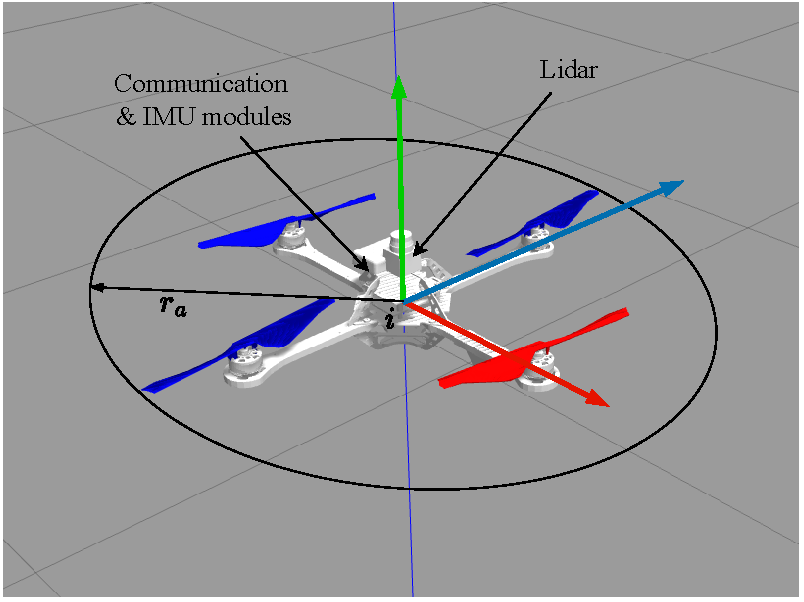
\includegraphics[width=\textwidth]{paper2/images/gazebo_uav.pdf}
    \caption{Gazebo SIL model}
    \label{fig:1gazebo_uav}
    \end{subfigure}
    \begin{subfigure}[b]{0.44\textwidth}
    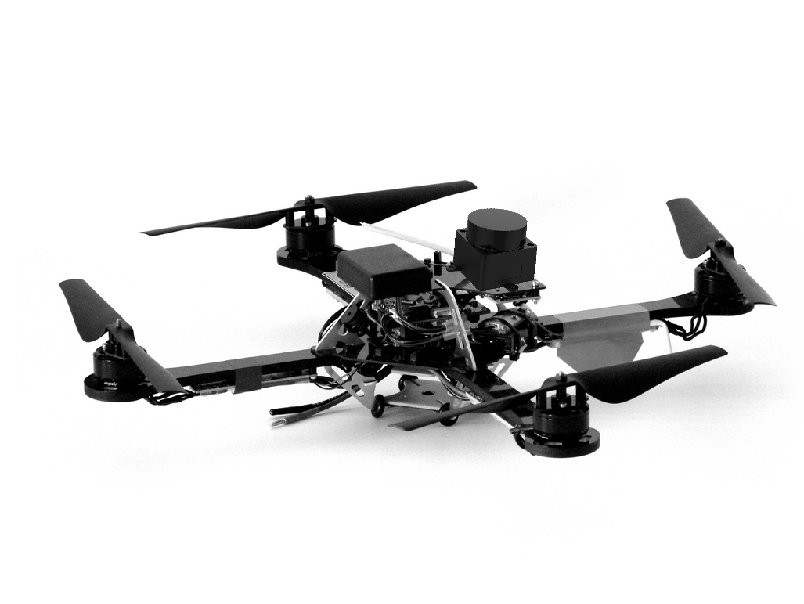
\includegraphics[width=\textwidth]{paper2/images/hummingbird.pdf}
    \caption{Real UAV model \cite{Furrer2016,Bui2022}}
    \label{fig:1gazebo_real}
    \end{subfigure}
    \caption{Used Hummingbird UAV model}
    \label{fig:1gazebo_setup}
\end{figure*}

\begin{figure*}[h!]
    \centering
    \begin{subfigure}[b]{0.495\textwidth}
    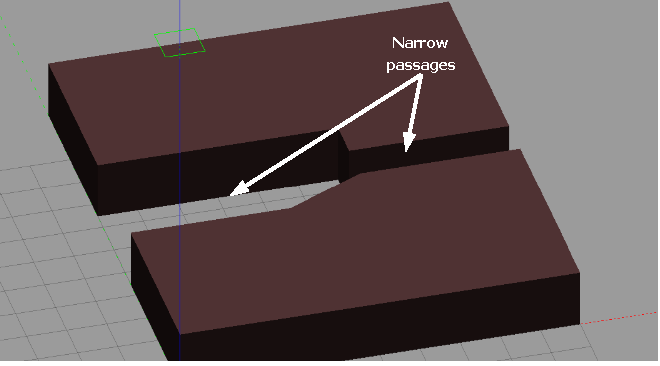
\includegraphics[width=\textwidth]{paper2/images/gazebo_env.pdf}
    \caption{The Gazebo environment}
    \end{subfigure}
    \begin{subfigure}[b]{0.40\textwidth}
    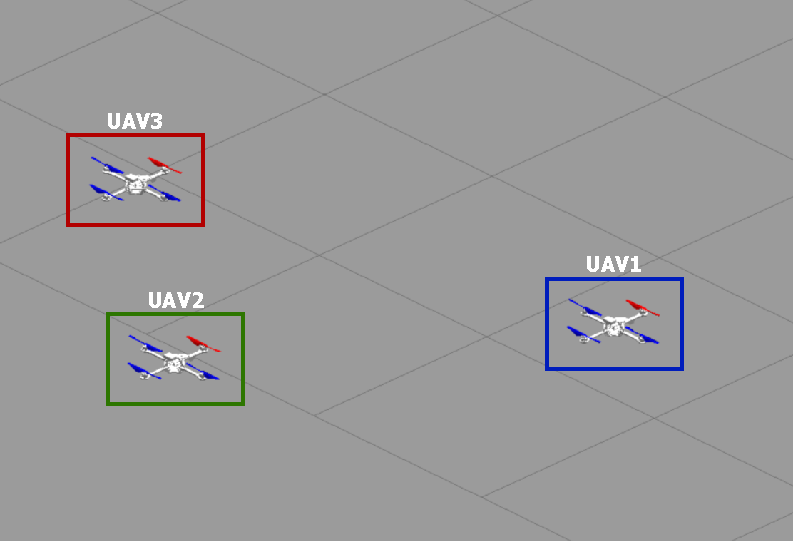
\includegraphics[width=\textwidth]{paper2/images/gazebo_init.pdf}
    \caption{Random initial positions}
    \label{fig:1gazebo_init}
    \end{subfigure}
    \caption{The environment in SIL test}
    \label{fig:1gazebo_env}
\end{figure*}

\begin{figure*}
    \centering
    \begin{subfigure}[b]{0.48\textwidth}
    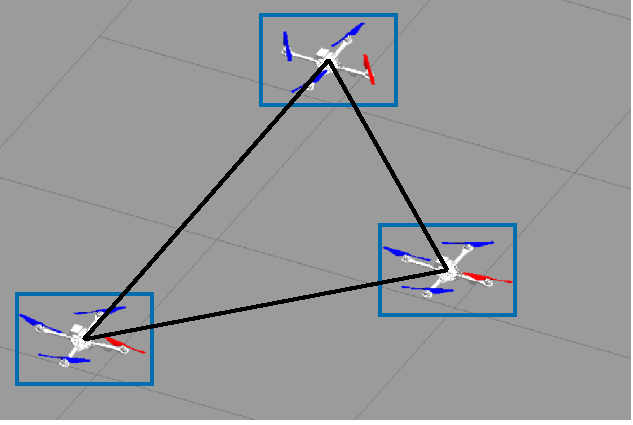
\includegraphics[width=\textwidth]{paper2/images/gazebo_res1.pdf}
    \caption{Maintain triangle formation from random}
    \label{fig:1gazebo_1}
    \end{subfigure}
    \begin{subfigure}[b]{0.48\textwidth}
    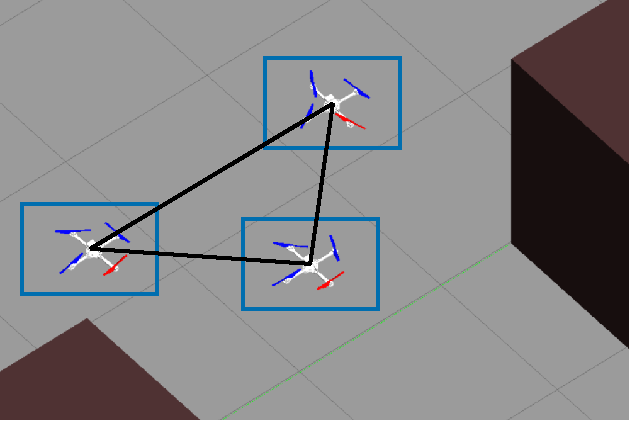
\includegraphics[width=\textwidth]{paper2/images/gazebo_res2.pdf}
    \caption{Small-scaled triangle formation}
    \label{fig:1gazebo_2}
    \end{subfigure}
    \begin{subfigure}[b]{0.48\textwidth}
    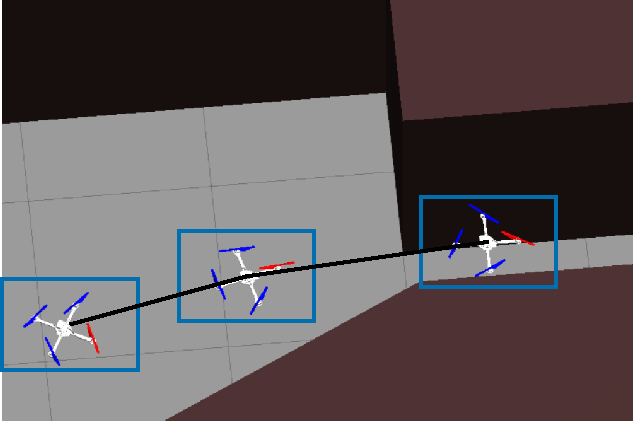
\includegraphics[width=\textwidth]{paper2/images/gazebo_res3.pdf}
    \caption{Transform to line formation}
    \label{fig:1gazebo_3}
    \end{subfigure}
    \begin{subfigure}[b]{0.48\textwidth}
    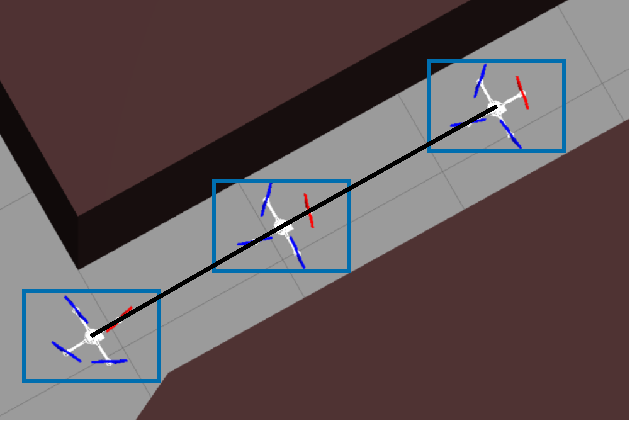
\includegraphics[width=\textwidth]{paper2/images/gazebo_res4.pdf}
    \caption{Line formation}
    \label{fig:1gazebo_4}
    \end{subfigure}
    \begin{subfigure}[b]{0.48\textwidth}
    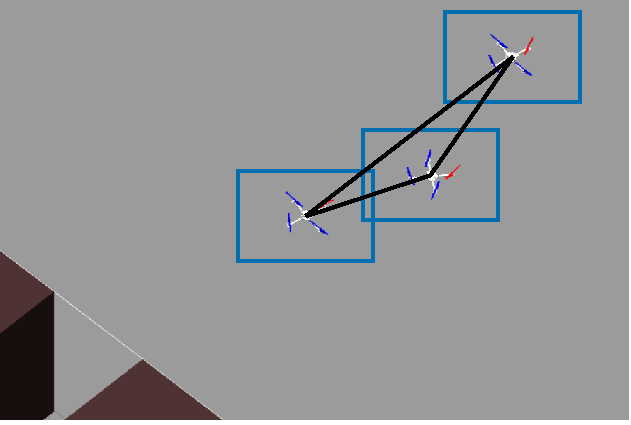
\includegraphics[width=\textwidth]{paper2/images/gazebo_res5.pdf}
    \caption{Transform back to triangle formation}
    \label{fig:1gazebo_5}
    \end{subfigure}
    \begin{subfigure}[b]{0.48\textwidth}
    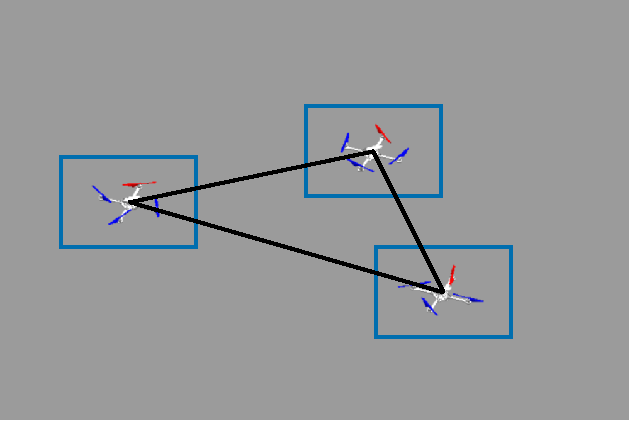
\includegraphics[width=\textwidth]{paper2/images/gazebo_res6.pdf}
    \caption{Original triangle formation}
    \label{fig:1gazebo_6}
    \end{subfigure}
    \caption{Validation results captured in the SIL Gazebo}
    \label{fig:1gazebo_result}
\end{figure*}

\begin{figure*}
    \centering
    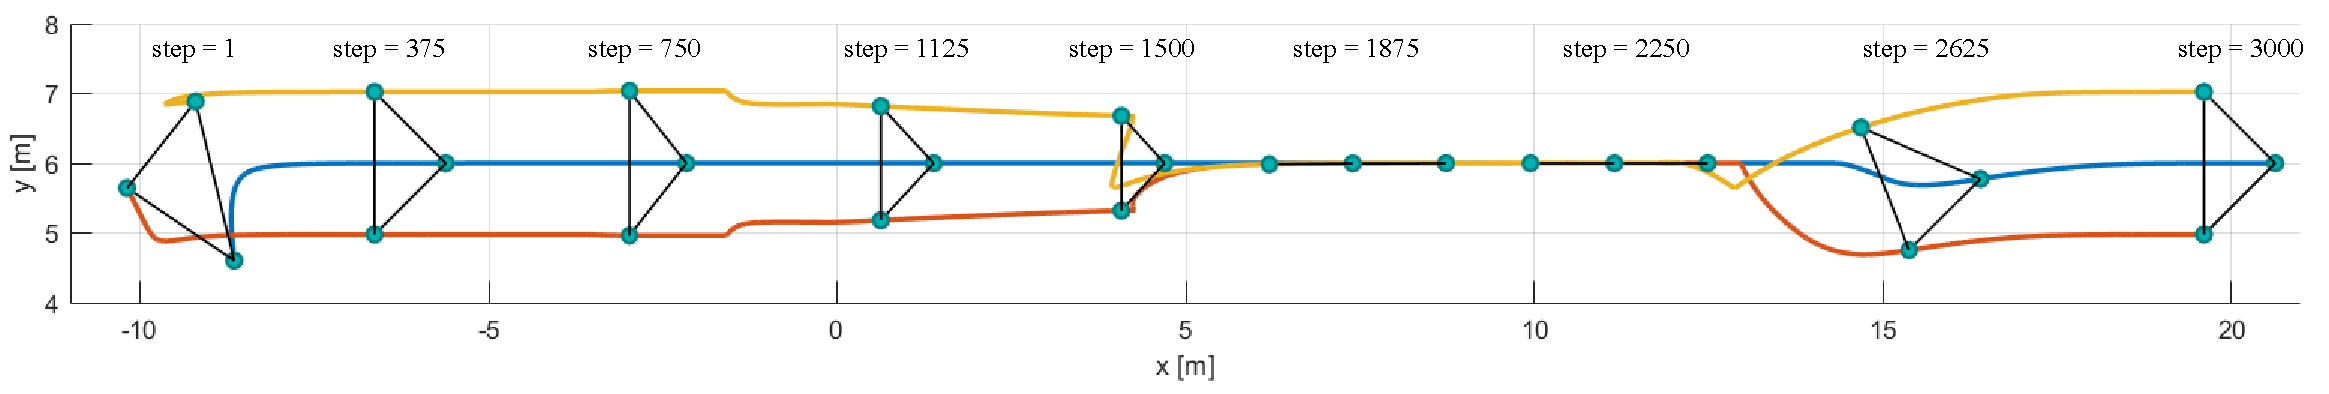
\includegraphics[width=\textwidth]{paper2/images/gazebo_path.pdf}
    \caption{The recorded paths of three UAV in the SIL test (Top view)}
    \label{fig:1gazebo_path}
\end{figure*}

To evaluate the applicability of the proposed system, we have conducted a software-in-the-loop (SIL) validation that involves navigating UAV formation pass through a confined space, which only focuses on a narrow tunnel-like environment in a Gazebo\footnote{Gazebo experiment video: {\fontfamily{qcr}\selectfont
\url{https://youtu.be/AIAAzRiIepg}}}. The used UAV model is a Hummingbird quadrotor developed based on Gazebo-based RotorS simulator~\cite{Furrer2016}, as described in Fig.~\ref{fig:1gazebo_uav}. We set up three UAVs in the experiment with random positions, as shown in Fig.~\ref{fig:1gazebo_init}. The environment in the SIL test includes two large obstacles, forming a width-varying tunnel, as depicted in Figure \ref{fig:1gazebo_env}.

Fig.~\ref{fig:1gazebo_result} presented the formation moving captured in the experiment. Moreover, the paths of three UAVs in the SIL test are recorded and are depicted in Fig.~\ref{fig:1gazebo_path}. At the beginning of the motion (step 1), three UAVs are in the random position. They then move to form the desired triangle formation (steps 375 - 750), as shown in Fig.~\ref{fig:1gazebo_1}. When sensing the narrow passage, the formation shrinks to safely move through the passage (steps 1125 - 1500), as shown in Fig.~\ref{fig:1gazebo_2}. When the narrow space is not suitable for the original formation, the formation transforms to the straight line formation as Fig.~\ref{fig:1gazebo_3} and then passes through the space with the line formation (steps 1875 - 2550), as Fig.~\ref{fig:1gazebo_4}. Once the UAV senses enough space in the environment to maintain its original formation, the formation transforms back to the origin shape in Fig.~\ref{fig:1gazebo_5} and moves to the target in Fig.~\ref{fig:1gazebo_6} (steps 2625 - 3000). The experiment demonstrates that the proposed \textit{EFRC} strategy successfully navigates the UAVs' formation to the target by passing through the narrow passage.

% \subsection{Discussion}
% Through simulation, validation, comparative statistics, and SIL testing, it is clear that our proposed method is capable of navigating the formation ensuring configuration, safety, and optimality for robot operation in narrow space environment.

% The proposed strategy provides flexibility for the robot formation to move safely through narrow space environments with numerous of formation configuration the ability to scale, rotate, and transform into a line configuration based on the perception of the environment depicted in Figure \ref{fig:1path}.

% The proposed algorithm also ensures scalability across various robot quantities within the formation, as presented in Figure \ref{fig:1path}. As long as the robots adhere to the specified configuration, the strategy offers the flexibility to navigate through narrow environments effectively.

% In our design, the formation maintenance and tailgating behaviors are proven to be stable through Lyapunov's theorem (see Appendix \ref{app:uf} and Appendix \ref{app:ut}), which proves that the system errors will converge to zero, as provided in Figure \ref{fig:1error}. Their convergence speed can be controlled through the parameters, $k_f$, $k_t$.

% On another note, our proposed strategy brings forth the capability to swiftly respond to environmental variations and traverse narrow spaces securely. Nonetheless, the transitions between states and abrupt alterations in formation size may result in occasional movement disruptions (see \textit{order} metric in Figure \ref{fig:1metric}). In such instances, employing control techniques like fuzzy logic or neural networks can be employed to improve the overall fluidity of formation movement.
\section{Conclusion}\label{sec5}
In this study, we have presented an event-based reconfiguration control to navigate a time-varying robot formation through narrow spaces across various environmental settings, including forest-like and tunnel-like terrains. The proposed strategy is constructed via several behaviors, which leverage the artificial potential field, which brings t to facilitate implementation. The controller includes two modes, \textit{``formation''} and \textit{``tailgating''}, and a scaling factor that enables the TVF to adapt its shape based on observed environmental conditions. The stability of the proposed approach is also demonstrated via the Lyapunov theorem. Evaluation results show that the proposed controller effectively navigates complex environments, achieving superior control performance in most metrics compared to other established methods. Additionally, software-in-the-loop tests verify the practicality and robustness of the proposed controller in real-world scenarios.

